% Options for packages loaded elsewhere
\PassOptionsToPackage{unicode}{hyperref}
\PassOptionsToPackage{hyphens}{url}
%
\documentclass[
]{article}
\usepackage{amsmath,amssymb}
\usepackage{lmodern}
\usepackage{iftex}
\ifPDFTeX
  \usepackage[T1]{fontenc}
  \usepackage[utf8]{inputenc}
  \usepackage{textcomp} % provide euro and other symbols
\else % if luatex or xetex
  \usepackage{unicode-math}
  \defaultfontfeatures{Scale=MatchLowercase}
  \defaultfontfeatures[\rmfamily]{Ligatures=TeX,Scale=1}
\fi
% Use upquote if available, for straight quotes in verbatim environments
\IfFileExists{upquote.sty}{\usepackage{upquote}}{}
\IfFileExists{microtype.sty}{% use microtype if available
  \usepackage[]{microtype}
  \UseMicrotypeSet[protrusion]{basicmath} % disable protrusion for tt fonts
}{}
\makeatletter
\@ifundefined{KOMAClassName}{% if non-KOMA class
  \IfFileExists{parskip.sty}{%
    \usepackage{parskip}
  }{% else
    \setlength{\parindent}{0pt}
    \setlength{\parskip}{6pt plus 2pt minus 1pt}}
}{% if KOMA class
  \KOMAoptions{parskip=half}}
\makeatother
\usepackage{xcolor}
\IfFileExists{xurl.sty}{\usepackage{xurl}}{} % add URL line breaks if available
\IfFileExists{bookmark.sty}{\usepackage{bookmark}}{\usepackage{hyperref}}
\hypersetup{
  pdftitle={Supplementary material for ``Current status and prospects of R-packages for the design of experiments''},
  pdfauthor={Emi Tanaka; Dewi Amaliah},
  pdfkeywords={experimental design, CRAN task view, user interface},
  hidelinks,
  pdfcreator={LaTeX via pandoc}}
\urlstyle{same} % disable monospaced font for URLs
\usepackage[margin=1in]{geometry}
\usepackage{longtable,booktabs,array}
\usepackage{calc} % for calculating minipage widths
% Correct order of tables after \paragraph or \subparagraph
\usepackage{etoolbox}
\makeatletter
\patchcmd\longtable{\par}{\if@noskipsec\mbox{}\fi\par}{}{}
\makeatother
% Allow footnotes in longtable head/foot
\IfFileExists{footnotehyper.sty}{\usepackage{footnotehyper}}{\usepackage{footnote}}
\makesavenoteenv{longtable}
\usepackage{graphicx}
\makeatletter
\def\maxwidth{\ifdim\Gin@nat@width>\linewidth\linewidth\else\Gin@nat@width\fi}
\def\maxheight{\ifdim\Gin@nat@height>\textheight\textheight\else\Gin@nat@height\fi}
\makeatother
% Scale images if necessary, so that they will not overflow the page
% margins by default, and it is still possible to overwrite the defaults
% using explicit options in \includegraphics[width, height, ...]{}
\setkeys{Gin}{width=\maxwidth,height=\maxheight,keepaspectratio}
% Set default figure placement to htbp
\makeatletter
\def\fps@figure{htbp}
\makeatother
\setlength{\emergencystretch}{3em} % prevent overfull lines
\providecommand{\tightlist}{%
  \setlength{\itemsep}{0pt}\setlength{\parskip}{0pt}}
\setcounter{secnumdepth}{5}
\usepackage{colortbl}
\usepackage{bera}
\usepackage{xcolor}
\usepackage{hyperref}
\usepackage{booktabs}
\usepackage[utf8]{inputenc}
\usepackage{caption}
\renewcommand{\figurename}{Figure S}
\makeatletter
\def\fnum@figure{\figurename\thefigure}
\makeatother
\renewcommand{\tablename}{Table S}
\makeatletter
\def\fnum@table{\tablename\thetable}
\makeatother

\usepackage{bera}
\ifLuaTeX
  \usepackage{selnolig}  % disable illegal ligatures
\fi
\usepackage[]{biblatex}
\addbibresource{pkgs.bib}

\title{Supplementary material for ``Current status and prospects of R-packages for the design of experiments''}
\author{Emi Tanaka \and Dewi Amaliah}
\date{}

\begin{document}
\maketitle

\begin{figure}[htbp]

{\centering 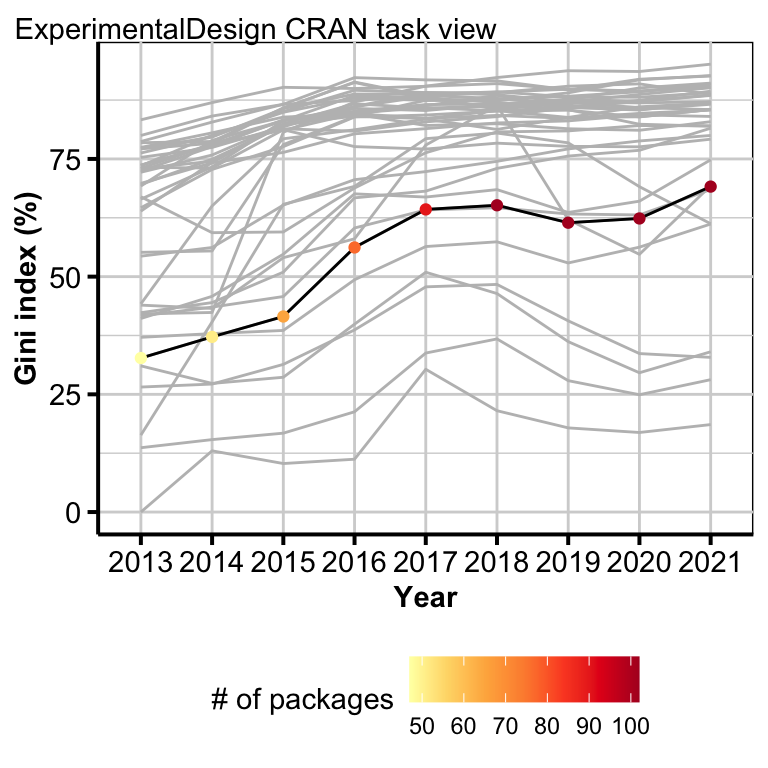
\includegraphics{figures/fig-gini-all-ctvs-1} 

}

\caption{The points show the Gini index of the download counts by year facetted by CRAN task view with the color showing the number of packages. The grey line shows the distribution of the Gini index across years for all other CRAN task views. The facets are ordered by increasing value of the Gini index in 2021.}\label{fig:fig-gini-all-ctvs}
\end{figure}

\begin{longtable}[t]{l>{\raggedright\arraybackslash}p{12em}>{\raggedleft\arraybackslash}p{5em}>{\raggedleft\arraybackslash}p{5em}>{\raggedleft\arraybackslash}p{5em}>{\raggedleft\arraybackslash}p{5em}}
\caption{\label{tab:ctv-summ-table}A summary table for the CRAN task view that shows in order: the name of the task view, the full topic name, the total of packages, the total number of contributors, the average number of contributors, and the intra-connectivity. The intra-connectivity measures the percentage of packages that depends, suggest or imports at least one other package within the same task view. A low intra-connectivity suggests that development within the topic mostly occur in silos whilst high  intra-connectivity suggests that there are more interactions within the topic. The row is ordered by the average number of contributors.}\\
\toprule
Name & Topic & \# of packages & Total \# of contributors & Average \# of contributors & Intra-connectivity (\%)\\
\midrule
\endfirsthead
\caption[]{\label{tab:ctv-summ-table}A summary table for the CRAN task view that shows in order: the name of the task view, the full topic name, the total of packages, the total number of contributors, the average number of contributors, and the intra-connectivity. The intra-connectivity measures the percentage of packages that depends, suggest or imports at least one other package within the same task view. A low intra-connectivity suggests that development within the topic mostly occur in silos whilst high  intra-connectivity suggests that there are more interactions within the topic. The row is ordered by the average number of contributors. \textit{(continued)}}\\
\toprule
Name & Topic & \# of packages & Total \# of contributors & Average \# of contributors & Intra-connectivity (\%)\\
\midrule
\endhead
\midrule
\multicolumn{6}{r@{}}{\textit{(Continued on next page...)}}\
\endfoot
\bottomrule
\endlastfoot
\cellcolor{gray!6}{ExperimentalDesign} & \cellcolor{gray!6}{Design of Experiments (DoE) \& Analysis of Experimental Data} & \cellcolor{gray!6}{112} & \cellcolor{gray!6}{211} & \cellcolor{gray!6}{2.27} & \cellcolor{gray!6}{29}\\
SportsAnalytics & Sports Analytics & 78 & 149 & 2.32 & 17\\
\cellcolor{gray!6}{MedicalImaging} & \cellcolor{gray!6}{Medical Image Analysis} & \cellcolor{gray!6}{32} & \cellcolor{gray!6}{53} & \cellcolor{gray!6}{2.44} & \cellcolor{gray!6}{44}\\
MetaAnalysis & Meta-Analysis & 157 & 351 & 2.63 & 43\\
\cellcolor{gray!6}{ChemPhys} & \cellcolor{gray!6}{Chemometrics and Computational Physics} & \cellcolor{gray!6}{75} & \cellcolor{gray!6}{162} & \cellcolor{gray!6}{2.65} & \cellcolor{gray!6}{28}\\
\addlinespace
ClinicalTrials & Clinical Trial Design, Monitoring, and Analysis & 59 & 141 & 2.76 & 31\\
\cellcolor{gray!6}{Distributions} & \cellcolor{gray!6}{Probability Distributions} & \cellcolor{gray!6}{257} & \cellcolor{gray!6}{597} & \cellcolor{gray!6}{2.88} & \cellcolor{gray!6}{45}\\
Survival & Survival Analysis & 239 & 558 & 2.92 & 73\\
\cellcolor{gray!6}{ExtremeValue} & \cellcolor{gray!6}{Extreme Value Analysis} & \cellcolor{gray!6}{37} & \cellcolor{gray!6}{89} & \cellcolor{gray!6}{2.95} & \cellcolor{gray!6}{41}\\
Optimization & Optimization and Mathematical Programming & 136 & 328 & 3.04 & 29\\
\addlinespace
\cellcolor{gray!6}{TimeSeries} & \cellcolor{gray!6}{Time Series Analysis} & \cellcolor{gray!6}{339} & \cellcolor{gray!6}{793} & \cellcolor{gray!6}{3.04} & \cellcolor{gray!6}{58}\\
OfficialStatistics & Official Statistics \& Survey Statistics & 131 & 325 & 3.06 & 40\\
\cellcolor{gray!6}{Hydrology} & \cellcolor{gray!6}{Hydrological Data and Modeling} & \cellcolor{gray!6}{100} & \cellcolor{gray!6}{252} & \cellcolor{gray!6}{3.09} & \cellcolor{gray!6}{24}\\
NumericalMathematics & Numerical Mathematics & 115 & 271 & 3.14 & 63\\
\cellcolor{gray!6}{Databases} & \cellcolor{gray!6}{Databases with R} & \cellcolor{gray!6}{43} & \cellcolor{gray!6}{95} & \cellcolor{gray!6}{3.23} & \cellcolor{gray!6}{77}\\
\addlinespace
WebTechnologies & Web Technologies and Services & 201 & 428 & 3.25 & 90\\
\cellcolor{gray!6}{NaturalLanguageProcessing} & \cellcolor{gray!6}{Natural Language Processing} & \cellcolor{gray!6}{56} & \cellcolor{gray!6}{130} & \cellcolor{gray!6}{3.30} & \cellcolor{gray!6}{62}\\
Bayesian & Bayesian Inference & 213 & 621 & 3.35 & 49\\
\cellcolor{gray!6}{FunctionalData} & \cellcolor{gray!6}{Functional Data Analysis} & \cellcolor{gray!6}{40} & \cellcolor{gray!6}{109} & \cellcolor{gray!6}{3.38} & \cellcolor{gray!6}{60}\\
Robust & Robust Statistical Methods & 59 & 136 & 3.41 & 75\\
\addlinespace
\cellcolor{gray!6}{Psychometrics} & \cellcolor{gray!6}{Psychometric Models and Methods} & \cellcolor{gray!6}{230} & \cellcolor{gray!6}{567} & \cellcolor{gray!6}{3.41} & \cellcolor{gray!6}{69}\\
Tracking & Processing and Analysis of Tracking Data & 46 & 149 & 3.46 & 48\\
\cellcolor{gray!6}{Cluster} & \cellcolor{gray!6}{Cluster Analysis \& Finite Mixture Models} & \cellcolor{gray!6}{108} & \cellcolor{gray!6}{305} & \cellcolor{gray!6}{3.47} & \cellcolor{gray!6}{39}\\
Econometrics & Econometrics & 152 & 363 & 3.50 & 81\\
\cellcolor{gray!6}{Finance} & \cellcolor{gray!6}{Empirical Finance} & \cellcolor{gray!6}{158} & \cellcolor{gray!6}{426} & \cellcolor{gray!6}{3.61} & \cellcolor{gray!6}{57}\\
\addlinespace
MissingData & Missing Data & 210 & 740 & 3.99 & 42\\
\cellcolor{gray!6}{SpatioTemporal} & \cellcolor{gray!6}{Handling and Analyzing Spatio-Temporal Data} & \cellcolor{gray!6}{81} & \cellcolor{gray!6}{269} & \cellcolor{gray!6}{4.04} & \cellcolor{gray!6}{70}\\
Spatial & Analysis of Spatial Data & 197 & 618 & 4.26 & 83\\
\cellcolor{gray!6}{GraphicalModels} & \cellcolor{gray!6}{Graphical Models} & \cellcolor{gray!6}{32} & \cellcolor{gray!6}{109} & \cellcolor{gray!6}{4.38} & \cellcolor{gray!6}{78}\\
Pharmacokinetics & Analysis of Pharmacokinetic Data & 29 & 109 & 4.55 & 21\\
\addlinespace
\cellcolor{gray!6}{HighPerformanceComputing} & \cellcolor{gray!6}{High-Performance and Parallel Computing with R} & \cellcolor{gray!6}{83} & \cellcolor{gray!6}{315} & \cellcolor{gray!6}{4.75} & \cellcolor{gray!6}{63}\\
DifferentialEquations & Differential Equations & 27 & 114 & 4.96 & 56\\
\cellcolor{gray!6}{Environmetrics} & \cellcolor{gray!6}{Analysis of Ecological and Environmental Data} & \cellcolor{gray!6}{93} & \cellcolor{gray!6}{383} & \cellcolor{gray!6}{5.02} & \cellcolor{gray!6}{74}\\
MachineLearning & Machine Learning \& Statistical Learning & 102 & 488 & 5.63 & 50\\
\cellcolor{gray!6}{TeachingStatistics} & \cellcolor{gray!6}{Teaching Statistics} & \cellcolor{gray!6}{46} & \cellcolor{gray!6}{236} & \cellcolor{gray!6}{6.35} & \cellcolor{gray!6}{57}\\
\addlinespace
ReproducibleResearch & Reproducible Research & 102 & 524 & 6.49 & 76\\
\cellcolor{gray!6}{ModelDeployment} & \cellcolor{gray!6}{Model Deployment with R} & \cellcolor{gray!6}{31} & \cellcolor{gray!6}{146} & \cellcolor{gray!6}{6.55} & \cellcolor{gray!6}{74}\\*
\end{longtable}



\hypertarget{session-information}{%
\section*{Session information}\label{session-information}}
\addcontentsline{toc}{section}{Session information}

\textbf{R version 4.1.2 (2021-11-01)}

\textbf{Platform:} x86\_64-apple-darwin17.0 (64-bit)

\textbf{locale:}
en\_AU.UTF-8\textbar\textbar en\_AU.UTF-8\textbar\textbar en\_AU.UTF-8\textbar\textbar C\textbar\textbar en\_AU.UTF-8\textbar\textbar en\_AU.UTF-8

\textbf{attached base packages:}

\textbf{other attached packages:}

\begin{itemize}
\tightlist
\item
  AsioHeaders(v.1.16.1-1)
\item
  BH(v.1.75.0-0)
\item
  DBI(v.1.1.1)
\item
  DT(v.0.23)
\item
  MASS(v.7.3-54)
\item
  Matrix(v.1.3-4)
\item
  R6(v.2.5.1)
\item
  RColorBrewer(v.1.1-2)
\item
  Rcpp(v.1.0.8)
\item
  RcppArmadillo(v.0.10.8.1.0)
\item
  RcppEigen(v.0.3.3.9.1)
\item
  SnowballC(v.0.7.0)
\item
  V8(v.4.2.0)
\item
  anytime(v.0.3.9)
\item
  askpass(v.1.1)
\item
  assertthat(v.0.2.1)
\item
  backports(v.1.3.0)
\item
  base64enc(v.0.1-3)
\item
  base64url(v.1.4)
\item
  beeswarm(v.0.4.0)
\item
  bit(v.4.0.4)
\item
  bit64(v.4.0.5)
\item
  blob(v.1.2.2)
\item
  bookdown(v.0.24)
\item
  broom(v.0.8.0)
\item
  bslib(v.0.3.1)
\item
  cachem(v.1.0.6)
\item
  callr(v.3.7.0)
\item
  cellranger(v.1.1.0)
\item
  cli(v.3.3.0)
\item
  clipr(v.0.7.1)
\item
  coda(v.0.19-4)
\item
  codetools(v.0.2-18)
\item
  colorspace(v.2.0-2)
\item
  commonmark(v.1.7)
\item
  cpp11(v.0.4.2)
\item
  cranlogs(v.2.1.1)
\item
  crayon(v.1.4.2)
\item
  crosstalk(v.1.2.0)
\item
  ctv(v.0.9-2)
\item
  curl(v.4.3.2)
\item
  data.table(v.1.14.2)
\item
  dbplyr(v.2.1.1)
\item
  digest(v.0.6.29)
\item
  distributional(v.0.2.2)
\item
  dplyr(v.1.0.9)
\item
  dtplyr(v.1.1.0)
\item
  ellipsis(v.0.3.2)
\item
  evaluate(v.0.14)
\item
  fable(v.0.3.1)
\item
  fabletools(v.0.3.1)
\item
  fansi(v.1.0.2)
\item
  farver(v.2.1.0)
\item
  fastmap(v.1.1.0)
\item
  feasts(v.0.2.2)
\item
  fontawesome(v.0.2.2)
\item
  forcats(v.0.5.1)
\item
  fs(v.1.5.2)
\item
  gargle(v.1.2.0)
\item
  generics(v.0.1.2)
\item
  ggbeeswarm(v.0.6.0)
\item
  ggforce(v.0.3.3)
\item
  ggnetwork(v.0.5.10)
\item
  ggnewscale(v.0.4.5)
\item
  ggplot2(v.3.3.5)
\item
  ggraph(v.2.0.5)
\item
  ggrepel(v.0.9.1)
\item
  ggwordcloud(v.0.5.0)
\item
  glue(v.1.6.1)
\item
  googledrive(v.2.0.0)
\item
  googlesheets4(v.1.0.0)
\item
  graphlayouts(v.0.8.0)
\item
  gridExtra(v.2.3)
\item
  gtable(v.0.3.0)
\item
  haven(v.2.4.3)
\item
  here(v.1.0.1)
\item
  highr(v.0.9)
\item
  hms(v.1.1.1)
\item
  htmltools(v.0.5.2)
\item
  htmlwidgets(v.1.5.4)
\item
  httpuv(v.1.6.3)
\item
  httr(v.1.4.2)
\item
  hunspell(v.3.0.1)
\item
  ids(v.1.0.1)
\item
  igraph(v.1.2.11)
\item
  ineq(v.0.2-13)
\item
  isoband(v.0.2.5)
\item
  janeaustenr(v.0.1.5)
\item
  jquerylib(v.0.1.4)
\item
  jsonlite(v.1.7.3)
\item
  kableExtra(v.1.3.4)
\item
  knitr(v.1.37)
\item
  labeling(v.0.4.2)
\item
  later(v.1.3.0)
\item
  lattice(v.0.20-45)
\item
  lazyeval(v.0.2.2)
\item
  lifecycle(v.1.0.1)
\item
  lubridate(v.1.8.0)
\item
  magrittr(v.2.0.2)
\item
  mgcv(v.1.8-38)
\item
  mime(v.0.12)
\item
  modelr(v.0.1.8)
\item
  munsell(v.0.5.0)
\item
  network(v.1.17.2)
\item
  networkD3(v.0.4)
\item
  nlme(v.3.1-153)
\item
  numDeriv(v.2016.8-1.1)
\item
  openssl(v.2.0.2)
\item
  pacman(v.0.5.1)
\item
  pagedown(v.0.16)
\item
  pander(v.0.6.6)
\item
  parsedate(v.1.3.0)
\item
  patchwork(v.1.1.1)
\item
  pillar(v.1.7.0)
\item
  pkgconfig(v.2.0.3)
\item
  pkgsearch(v.3.1.0)
\item
  plotly(v.4.10.0)
\item
  pluralize(v.0.2.0)
\item
  plyr(v.1.8.6)
\item
  png(v.0.1-7)
\item
  polyclip(v.1.10-0)
\item
  prettyunits(v.1.1.1)
\item
  processx(v.3.5.2)
\item
  progress(v.1.2.2)
\item
  progressr(v.0.9.0)
\item
  promises(v.1.2.0.1)
\item
  ps(v.1.6.0)
\item
  purrr(v.0.3.4)
\item
  qdapRegex(v.0.7.5)
\item
  rappdirs(v.0.3.3)
\item
  readr(v.2.1.2)
\item
  readxl(v.1.3.1)
\item
  rematch(v.1.0.1)
\item
  rematch2(v.2.1.2)
\item
  remotes(v.2.4.2)
\item
  renv(v.0.15.5)
\item
  reprex(v.2.0.1)
\item
  reshape(v.0.8.8)
\item
  rlang(v.1.0.2)
\item
  rmarkdown(v.2.11)
\item
  rprojroot(v.2.0.2)
\item
  rstudioapi(v.0.13)
\item
  rticles(v.0.22)
\item
  rvest(v.1.0.2)
\item
  sass(v.0.4.0)
\item
  scales(v.1.1.1)
\item
  selectr(v.0.4-2)
\item
  servr(v.0.24)
\item
  shiny(v.1.7.1)
\item
  slider(v.0.2.2)
\item
  sna(v.2.7)
\item
  sourcetools(v.0.1.7)
\item
  splitstackshape(v.1.4.8)
\item
  statnet.common(v.4.6.0)
\item
  stringi(v.1.7.6)
\item
  stringr(v.1.4.0)
\item
  svglite(v.2.0.0)
\item
  sys(v.3.4)
\item
  systemfonts(v.1.0.3)
\item
  tarchetypes(v.0.6.0)
\item
  targets(v.0.12.0)
\item
  tibble(v.3.1.6)
\item
  tidygraph(v.1.2.0)
\item
  tidyr(v.1.2.0)
\item
  tidyselect(v.1.1.2)
\item
  tidytext(v.0.3.2)
\item
  tidyverse(v.1.3.1)
\item
  tinytex(v.0.36)
\item
  tokenizers(v.0.2.1)
\item
  tsibble(v.1.1.0)
\item
  tweenr(v.1.0.2)
\item
  tzdb(v.0.2.0)
\item
  utf8(v.1.2.2)
\item
  uuid(v.1.0-3)
\item
  vctrs(v.0.4.1)
\item
  vipor(v.0.4.5)
\item
  viridis(v.0.6.2)
\item
  viridisLite(v.0.4.0)
\item
  visNetwork(v.2.1.0)
\item
  vroom(v.1.5.7)
\item
  warp(v.0.2.0)
\item
  webshot(v.0.5.2)
\item
  websocket(v.1.4.1)
\item
  withr(v.2.4.3)
\item
  xfun(v.0.29)
\item
  xml2(v.1.3.2)
\item
  xtable(v.1.8-4)
\item
  yaml(v.2.2.2)
\end{itemize}

\textbf{loaded via a namespace (and not attached):}

\begin{itemize}
\tightlist
\item
  utils(v.4.1.2)
\item
  tools(v.4.1.2)
\item
  compiler(v.4.1.2)
\item
  datasets(v.4.1.2)
\item
  base(v.4.1.2)
\item
  grDevices(v.4.1.2)
\item
  grid(v.4.1.2)
\item
  methods(v.4.1.2)
\item
  graphics(v.4.1.2)
\item
  stats(v.4.1.2)
\end{itemize}

\printbibliography

\end{document}
